\documentclass{article}
\usepackage{amssymb}
\usepackage[utf8]{inputenc}
\usepackage{mathtools}
\usepackage{indentfirst}
\usepackage{verbatim}
\usepackage{gensymb}
\usepackage{graphicx}


\title{Math}
\author{Nathan Ueda}
\date{January 2024}

\begin{document}

\maketitle

\section{Stochastic Matrices}
\subsection{Stochastic Matrices}
    \begin{itemize}
        \item Informal definition: A square matrix that represent 
        transitions between different random states. Elements within a 
        stochastic matrix represent probabilities. This implies that each 
        element must be nonnegative and each row must sum to 1.
        \item Formal definition: A matrix $ \Phi \in R^{N \times N} $ is a 
        stochastic matrix if:
        \begin{itemize}
            \item all elements are positive: $ \Phi_{ij} \ge 0 \text{ for 
            all } i,j $
            \item each row sums to 1: $ \Sigma_j \Phi_{ij} = 1 \text{ for 
            all } i $
        \end{itemize}
    \end{itemize}

\subsubsection{Intepretations}
\begin{itemize}
    \item $P(s_{t+1} = n | s_t = m) = \Phi_{mn} $: This says that the element
    $ \Phi_{mn} $ represents the probability of the next state, $ s_{t+1} $ 
    being equal to $ n $ given that the current state, $ s_t $ is the $ m $th 
    state for all possible states $ s \in \{1, \dots, N\} $.
\end{itemize}

\subsubsection{Examples}
\begin{enumerate}
    \item 3-State Markov Process: Stochastic Matrix $ \Phi = \begin{bmatrix}
        0.8 & 0.2 & 0 \\
        0 & 0 & 1 \\
        0.05 & 0.95 & 0 
        \end{bmatrix} $
        \begin{center}
            \centering
            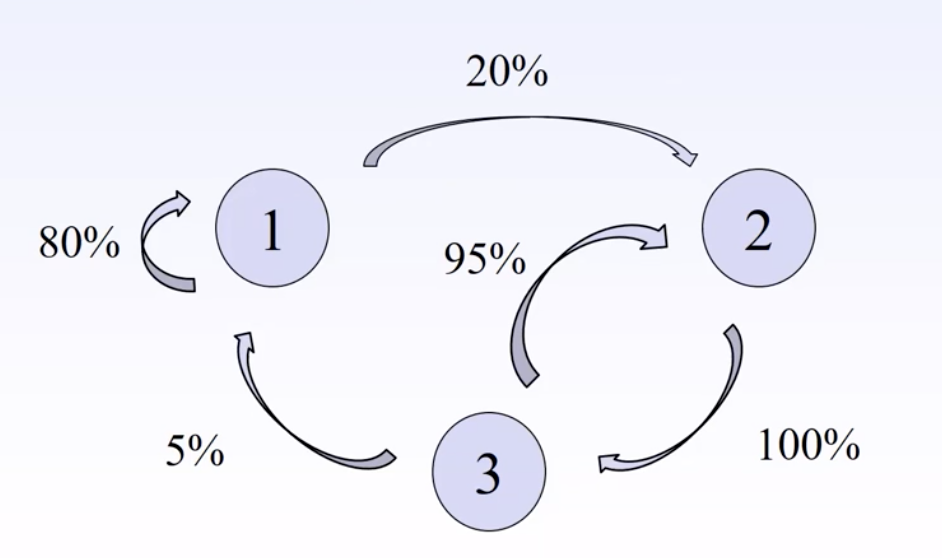
\includegraphics[width=0.8\textwidth]{imgs/stochastic_matrices1.png} \\
            \textit{Each node is a state. Each edge represents the probability of 
            transitioning from some state to another.}
        \end{center}
\end{enumerate}

\subsection{Discrete Kolmogorov Backward Equations}
\begin{itemize}
    \item Informal definition: 
    A formula to represent the expected value of some payoff function (i.e. for
    an option) depending upon what state we are in the future.
    \item Formal definition: For function $ F : \{ 1, \dots, N \}  \rightarrow R
    , $ define $ F(j) = f_j, f \in \mathbb{R}^N $.
    \begin{itemize}
        \item $ F $ is the `payoff function' and $ f_j $ is the payoff, given we 
        are in state $ j $ at some future specified time.
    \end{itemize}
\end{itemize}

\subsubsection{Intepretations}
\begin{enumerate}
    \item $ \Phi^2 = \Phi \Phi $: The transition probabilities between two 
    periods, $ t $ and $ t + 2 $.
    \item $ \Phi^n $: The transition probabilities between n periods, $ t $ and
    $ t + n $.
    \item $ {[\Phi^{T-t}]}_{ij} = P(s_T = j | s_t = i) $: The probability of 
    being in state $ j $ after $ t $ periods, given that we are in state $ i $
    currently (at time $ t $) is the $ ij $-th element of the stochastic matrix
    $ \Phi^{T-t} $.
    \item $ E[F(s_T) | s_t = j] = {[\Phi^{T-t}f]}_j $: The expected payoff at 
    period $ T $, given that we are currently in state $ s_t = j $ at period 
    $ t $, is the $ j $-th element of the vector resulting from taking the 
    product of $ \Phi^{T-t} $ and the payoff function $ f $. 
    \begin{itemize}
        \item $ {[\Phi^{T-t}f]}_j = \Phi_{j1}^{T-t} f_1 + \cdots + \Phi_{jN}^{T-t} f_N $
    \end{itemize}
\end{enumerate}

\subsubsection{Examples}
\begin{enumerate}
    \item 3-State Markov Process: Stochastic Matrix $ \Phi = \begin{bmatrix}
        0.8 & 0.2 & 0 \\
        0 & 0 & 1 \\
        0.05 & 0.95 & 0 
        \end{bmatrix} $, \\
        $ \Phi^2 = \begin{bmatrix}
            0.64 & 0.16 & 0.2 \\
            0.05 & 0.95 & 0 \\
            0.04 & 0.01 & 0.95 
            \end{bmatrix} $
    \begin{center}
        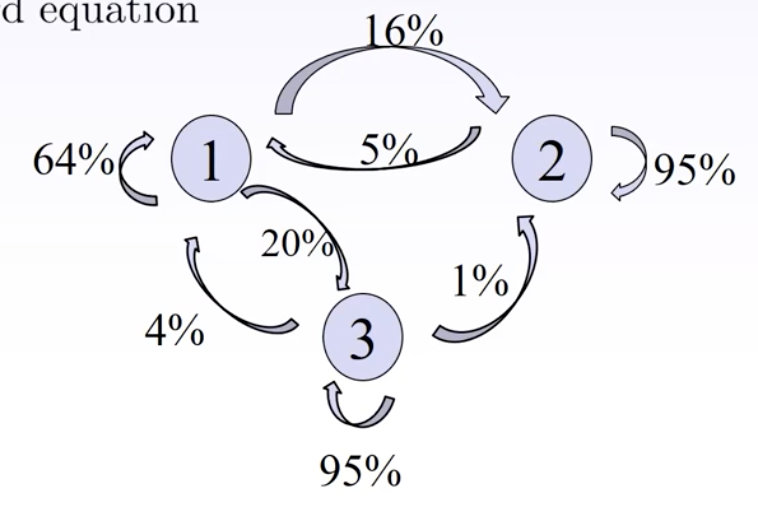
\includegraphics[width=0.8\textwidth]{imgs/stochastic_matrices2.png} \\
        \textit{Each node is a state. Each edge represents the probability of 
        ending up in the state at the end of the arrow, given we are in the 
        state at the tail of the arrow 2 periods prior.}
    \end{center}
\end{enumerate}

\subsection{Discrete Kolmogorov Forward Equations}
\begin{itemize}
    \item Informal definition: An equation useful in determining the distribution
    of us being in a specific state $ t $ periods into the future. 
    \item Formal definition: 
    \begin{itemize}
        \item Probability vector: a vector $ p \in \mathbb{R}^N $ such that:
        \begin{itemize}
            \item $ p_i \ge 0 $
            \item $ \Sigma_i p_i = 1 $
        \end{itemize}
        \item Stationary distribution: a probability vector for a stochastic
        matrix, $ \Phi $, such that $ p = \Phi^* p $ (i.e. $ p $ is a left
        eigenvector of $ \Phi^* $ with an eigenvalue of 1) ($ \Phi^* $ is used 
        to denote the transpose).
        \item Discrete Kolmogorov Forward Equation: if the probability vector at
        $ t $ is $ p^t $, then at time $ T $, the probability vector for being
        in any given state is $ {(\Phi^*)}^{T-t}p^t $.
    \end{itemize}
    \item To ensure a stochastic matrix has a unique stationary distribution, 
    two criteria must be fulfilled:
    \begin{enumerate}
        \item The matrix must be \textbf{irreducible}. As stochastic matrix is said to be 
        irreducible if, for each $ i,j $, there exists $ k > 0 $ such that $ 
        {(\Phi^k)}_{ij} > 0$. In other words, there exists some path that has a 
        non-zero probability between any two states.
        \item The Markov chain is \textbf{aperiodic}. The \textbf{period} of 
        state $ i $, is $ k_i $, where $ k_i $ is the greatest common divisor of 
        the set $ \{n | {(\Phi^n)}_{ii} > 0\} $. If $ k_i = 1 $ for $ i = 1, 
        \dots, n $, then $ \Phi $ is aperiodic. In other words, to be aperiodic 
        means there is no cyclicality in the number of steps it takes to get 
        back to some starting state. 
    \item \textbf{Perron-Frobenius Theorem}: Consider an irreducible, aperiodic
    stochastic matrix $ \Phi $. Then $ \Phi $ has a unique stationary 
    distribution with strictly positive elements.
    \begin{itemize}
        \item All other left eigvenvalues of $ \Phi, \lambda_2, \dots, 
        \lambda_N, $ have $ |\lambda_i| < 1 $.
        \item All other left eigenvectors of $ \Phi $ have at least one 
        nonpositive element. 
    \end{itemize}
    \end{enumerate}
\end{itemize}
\subsubsection{Intepretations}
\begin{enumerate}
    \item $ \Phi^{1000} = \begin{bmatrix}
        0.111 & 0.444 & 0.444 \\
        0.111 & 0.444 & 0.444 \\
        0.111 & 0.444 & 0.444
        \end{bmatrix} $: This is the transition matrix 1000 periods into the 
        future. Each column has the same values. This means regardless of which
        state we start in, we have the same probability of ending up in any
        state 1000 periods later. This implies there is a limiting distribution 
        $ \textbf{p} = (0.111, 0.444, 0.444)' $ regardless of the initial state. 
        Note: there is not always a limiting distribution. 
\end{enumerate}

\subsection{Multidimensional Calculus}
\subsubsection{Intermediate Value Therorem}
\begin{enumerate}
    \item Informal Definition: Given some continuous function that maps a point 
    $ a \rightarrow f(a) $ and $ b \rightarrow f(b) $, then there exists some 
    point $ s $ where $ a \le s \le b $, such that $ f(a) \le f(s) \le f(b) $.
    \item Formal Definition: Consider a continuous function $ f: [a,b] 
    \rightarrow R $ and a number $ x \in [f(a), f(b)] $. Then $ \exists\ s \in 
    [a, b] $ such that $ f(s) = x $.  
    \begin{center}
        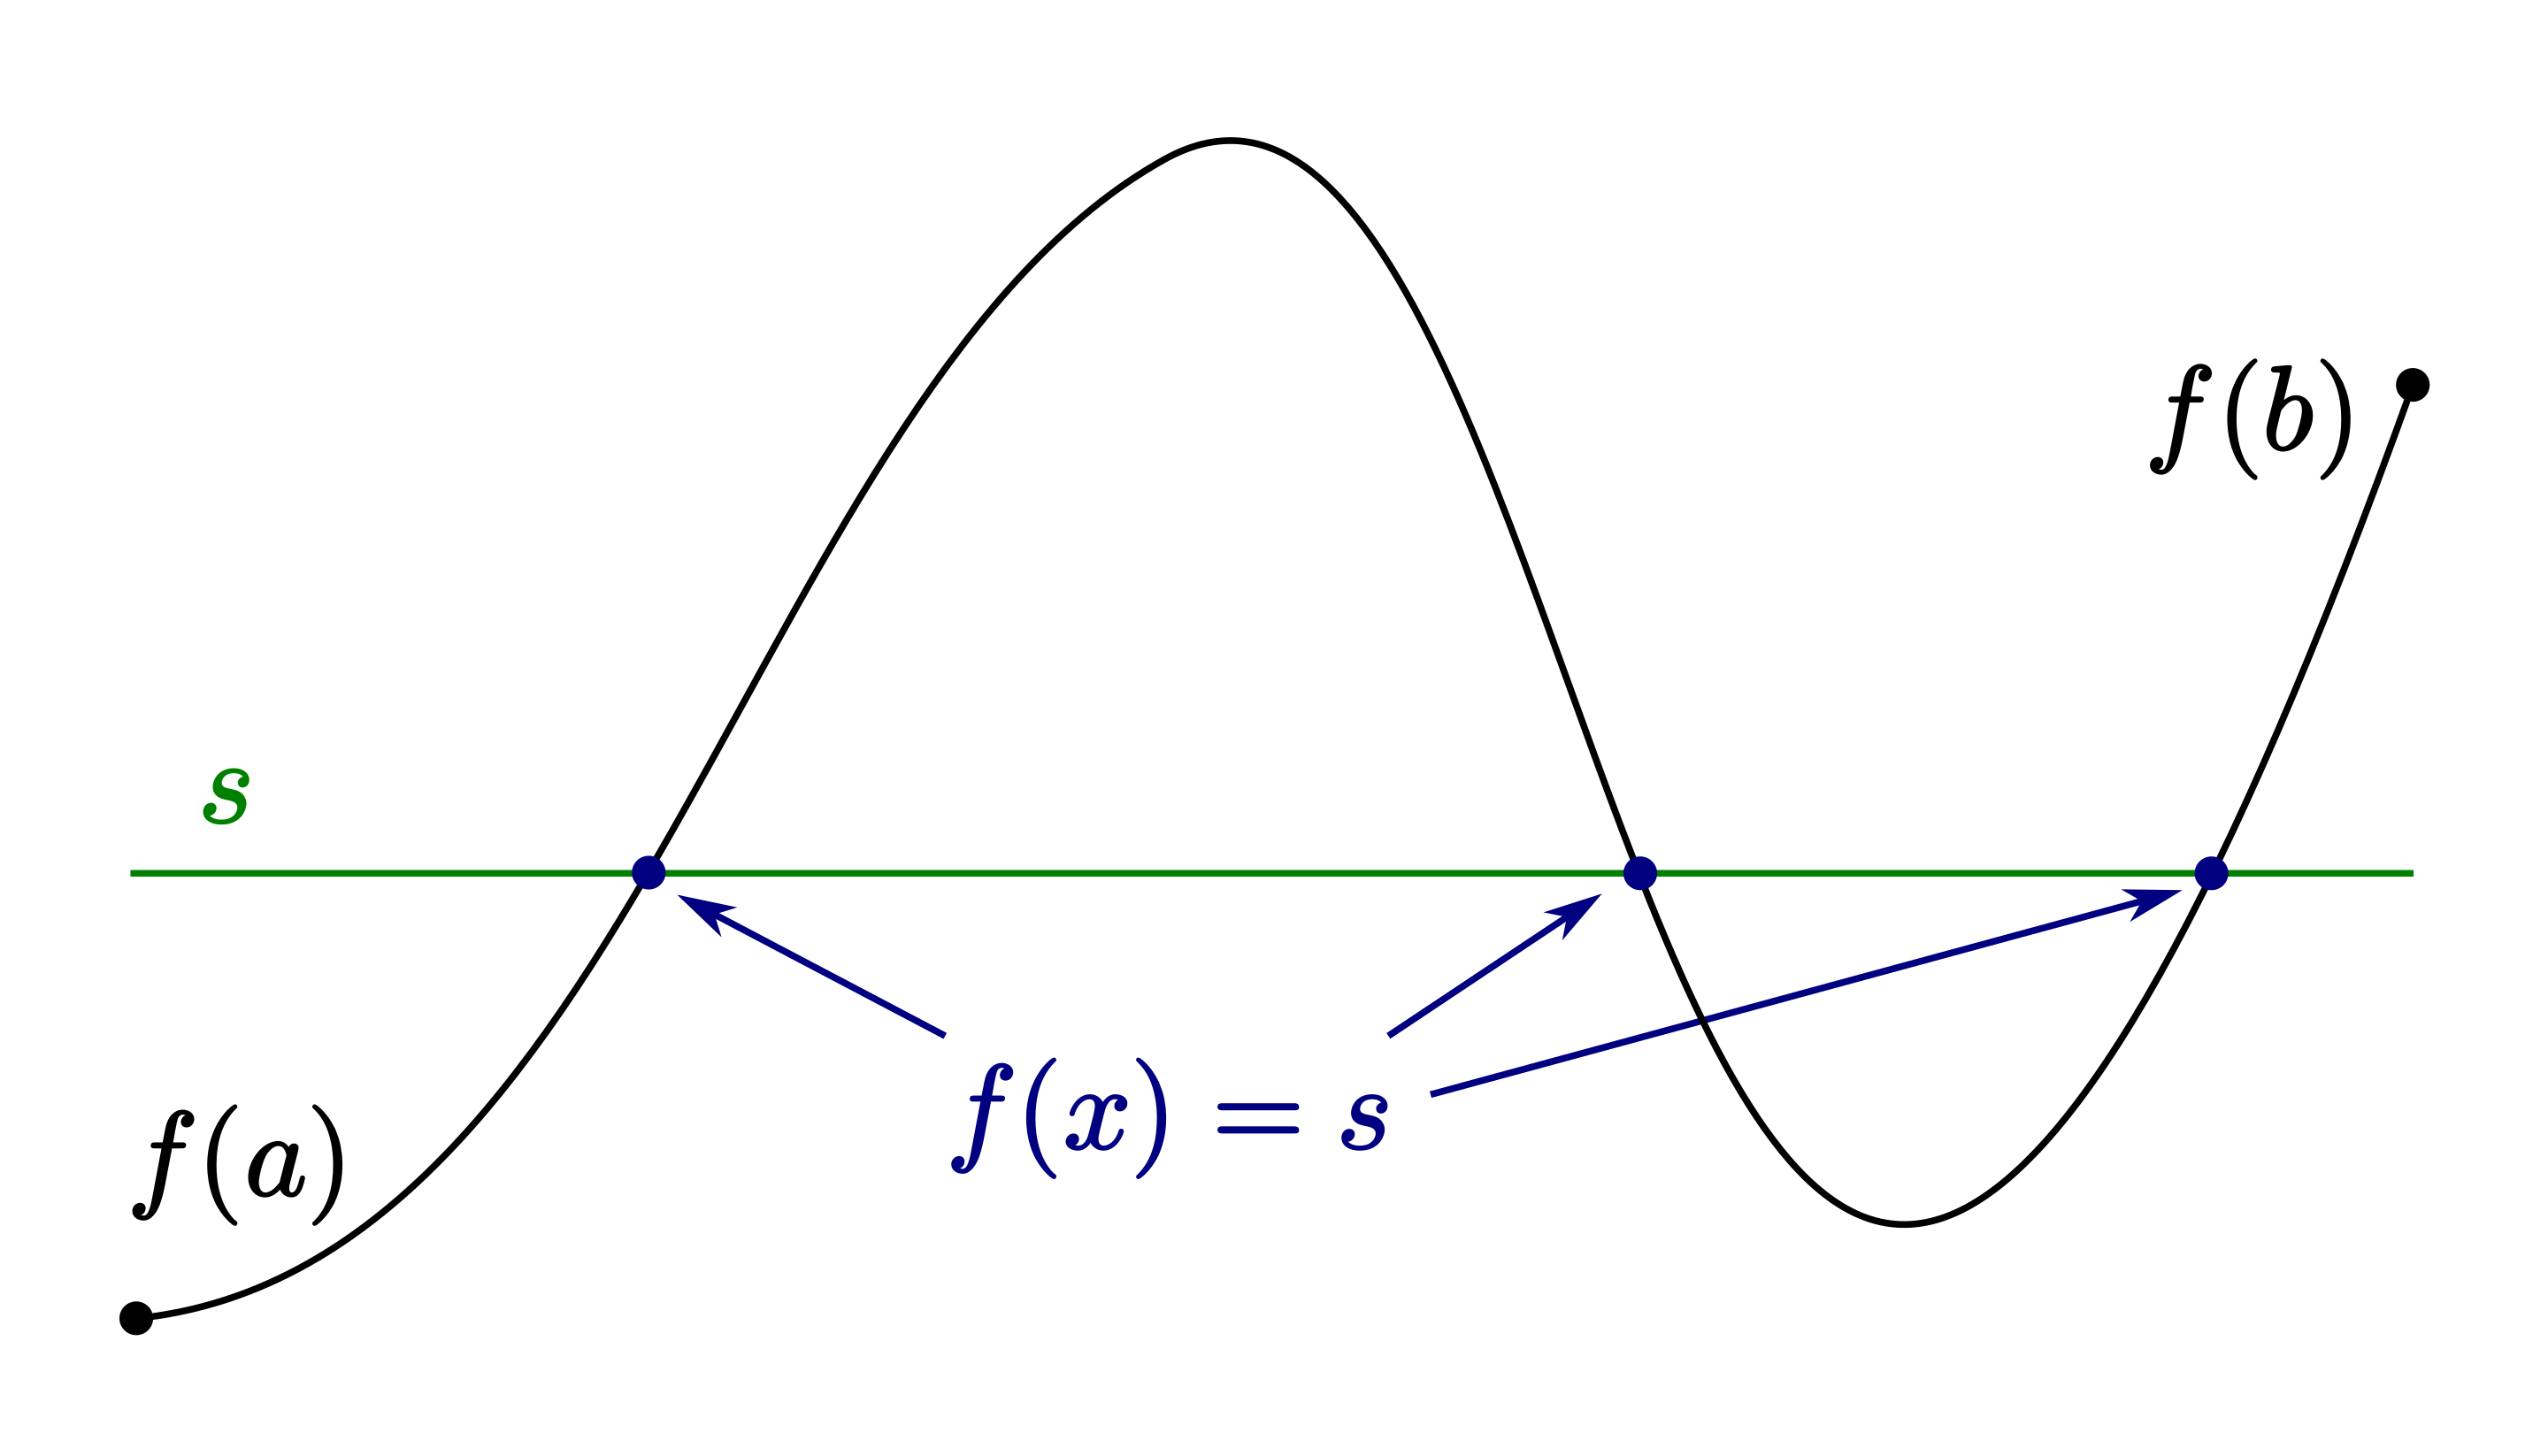
\includegraphics[width=0.8\textwidth]{imgs/intermediate_value_thm.png} \\
    \end{center}
\end{enumerate}

\subsubsection{Contraction Mapping Theorem}
\begin{itemize}
    \item Informal Definition: A theorem that, if it holds, guarantees the 
    existence and uniqueness of a fixed point for a complete metric space. 
    \item Formal Definition: If $ X $ is a complete metric space and $ f: X 
    \rightarrow X $ is a contraction, then $ f $ has a unique fixed point $ x 
    \in X $. 
    \begin{itemize}
        \item A function $ f: X \rightarrow X $ is called a contraction if $
        d(f(x), f(y)) \le k \times d(x, y) \ \forall \ x,y \in X $, for some $
        k < 1 $. In other words, a function is a contraction if it decreases 
        distances between every pair of points. 
    \end{itemize}
\end{itemize}

\subsubsection{Partial Derivatives}
\begin{itemize}
    \item For a function $ f : \mathbb{R}^N \rightarrow R^M$, define the partial
    derivative: $ a_{nm} = \frac{\partial f{(x)}_m}{\partial x_n} = D_n{(f)}_m $.
    \item Theorem: If $ f $ is differentiable at a point $ x $, then the total 
    derivative is given by $ A \in R^{M \times N} $, where $ A = \begin{bmatrix}
        a_{11} & \cdots & a_{1N} \\
        \vdots & \ddots & \vdots \\
        a_{M1} & \cdots & a_{MN} 
        \end{bmatrix} $
    \item Caveat: Partial derivatives may exist even when the total derivative 
    does not.
    \item When $ M=1  $, we have a gradient operator: $ \nabla f = \begin{bmatrix}
        \frac{\partial f}{\partial x_1} \\
        \vdots \\
        \frac{\partial f}{\partial x_N} \\
        \end{bmatrix}^T $
    \item The Hessian matrix is a square matrix of second order partial derivatives:
    $ H = \nabla^2 = \begin{bmatrix}
        \frac{\partial^2 f}{\partial x_1^2} && \frac{\partial^2 f}{\partial x_1 \partial x_2} && \cdots && \frac{\partial^2 f}{\partial x_1 \partial x_n} \\
        \frac{\partial^2 f}{\partial x_2 \partial x_1} && \frac{\partial^2 f}{\partial x_2^2} && \cdots && \frac{\partial^2 f}{\partial x_2 \partial x_n} \\
        \vdots && \vdots && \ddots && \vdots \\
        \frac{\partial^2 f}{\partial x_n \partial x_1} && \frac{\partial^2 f}{\partial x_n \partial x_2} && \cdots && \frac{\partial^2 f}{\partial x_n^2} \\
        \end{bmatrix} $
\end{itemize}

\subsection{Optimization}
\subsubsection{Univariate General Existence Result Theorem}
\begin{itemize}
    \item Informal Definition: If we can make a few assumptions about a function,
    namely that it has a well-defined domain, is closed, and is bounded, then 
    the existence of a maximum and a minimum to a function is guaranteed.
    \item Formal Definition: Suppose $ f: E \rightarrow R $ is a continuous
    function from a closed, bounded set $ E \subset \mathbb{R}^N $. Define:
    \begin{itemize}
        \item $ M = \underset{x \in E}{\sup} f(x) $
        \item $ m = \underset{x \in E}{\inf} f(x) $
    \end{itemize}
    Then there exists points $ \underbar{x} \in E, \bar{x} \in E $ such that 
    $ f(\underbar{x}) = m $ and $ f(\bar{x} = M) $ (theorem 4.16 in Rudin).
\end{itemize}

\subsubsection{Convex Set}
\begin{itemize}
    \item Informal Definition: A set is \textbf{convex} if for every $ \lambda \in (0,1) $
    and any two points $ x, y $ in the set, the weighted average that puts
    $ \lambda $ weight on $ x $ and $ 1 - \lambda $ weight on $ y $ is also in 
    the set. 
    \item Formal Definition: A set $ E \subset \mathbb{R}^N $ is said to be 
    \textbf{convex} if $ \forall \lambda \in (0,1), \forall x \in E, \forall y
    \in E: \lambda x + (1 - \lambda)y \in E $
    \begin{center}
        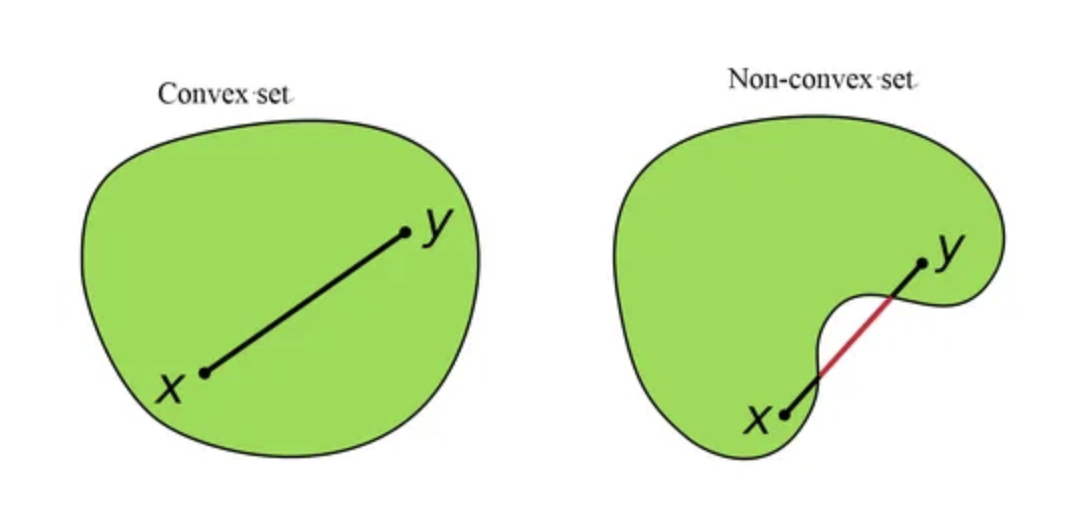
\includegraphics[width=0.8\textwidth]{imgs/convex.png} \\
    \end{center}
\end{itemize}
\subsubsection{Concave and Convex Functions}
\begin{itemize}
    \item Informal Definition: A function on a convex set is 
    \begin{itemize}
        \item \textbf{concave} if for every $ \lambda \in (0,1) $
        and any two points $ x, y $ in the set, the function evaluated at $ 
        \lambda x + (1 - \lambda)y $ (a point between x and y) is greater than 
        or equal to the weighted average of the values at those points.
        \item \textbf{convex} if for every $ \lambda \in (0,1) $
        and any two points $ x, y $ in the set, the function evaluated at $ 
        \lambda x + (1 - \lambda)y $ (a point between x and y) is less than or 
        equal to the weighted average of the values at those points.
        \item \textbf{stricly concave} if for every $ \lambda \in (0,1) $
        and any two points $ x, y $ in the set, the function evaluated at $ 
        \lambda x + (1 - \lambda)y $ (a point between x and y) is greater than 
        to the weighted average of the values at those points.
        \item \textbf{strictly convex} if for every $ \lambda \in (0,1) $
        and any two points $ x, y $ in the set, the function evaluated at $ 
        \lambda x + (1 - \lambda)y $ (a point between x and y) is less than to 
        the weighted average of the values at those points.
    \end{itemize}
    \item Formal Definition: A function $ f : E \rightarrow \mathbb{R}^N $,
    where $ E \subset \mathbb{R}^N $ is convex, is said to be:
    \begin{itemize}
        \item \textbf{concave} if $ \forall \lambda \in (0, 1), x, y \in E, 
        f(\lambda x + (1 - \lambda)y) \ge \lambda f(x) + (1 - \lambda) f(y) $
        \item \textbf{convex} if $ \forall \lambda \in (0, 1), x, y \in E, 
        f(\lambda x + (1 - \lambda)y) \le \lambda f(x) + (1 - \lambda) f(y) $
        \item \textbf{stricly concave}: replace $ \ge $ with $ > $
        \item \textbf{stricly convex}: replace $ \le $ with $ < $
    \end{itemize}
    \begin{center}
        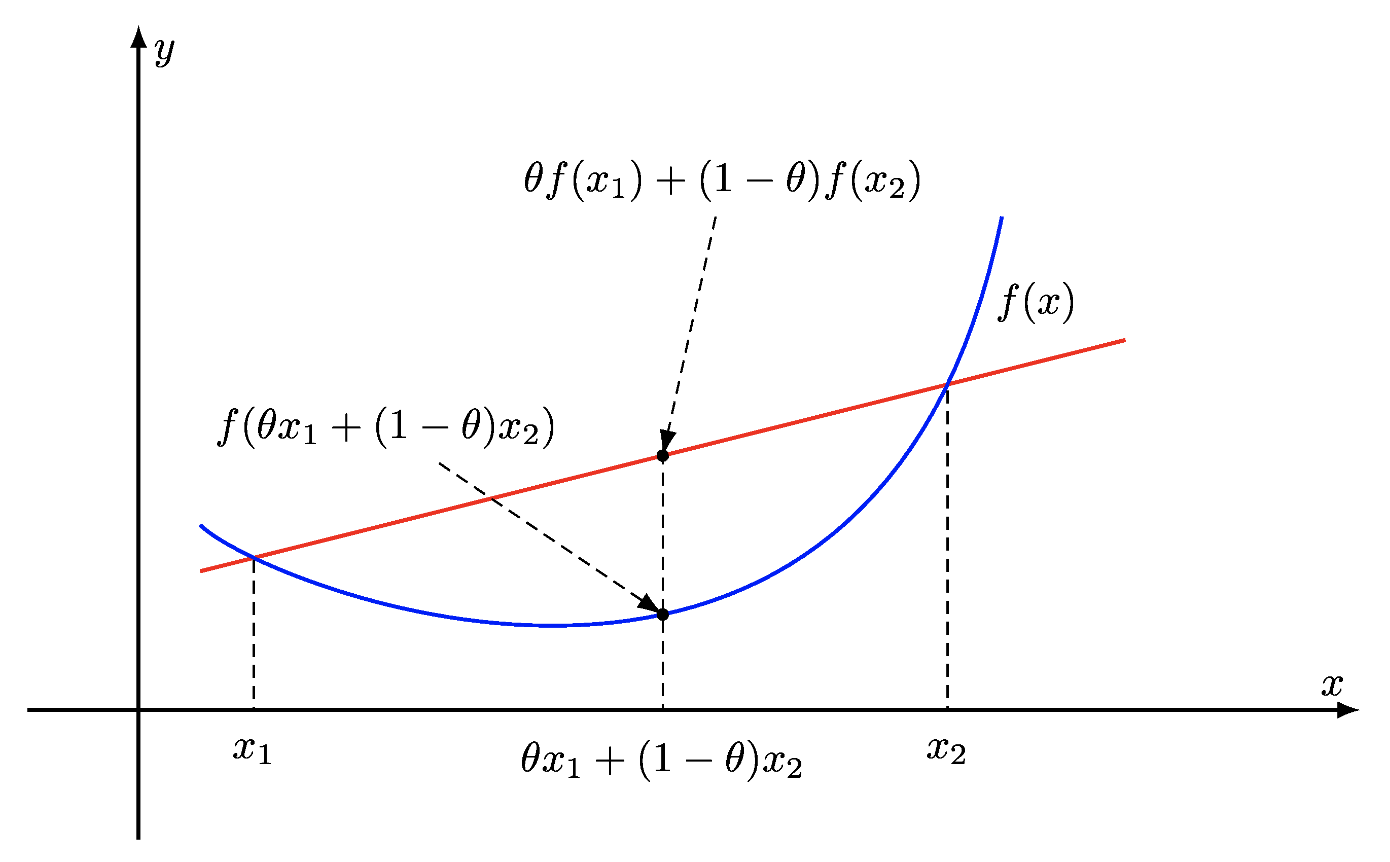
\includegraphics[width=0.9\textwidth]{imgs/convex_function.png} \\
        \textit{Graph of a convex function. The line segment between any two
        points on the graph lies above the graph.}
    \end{center}
    \begin{center}
        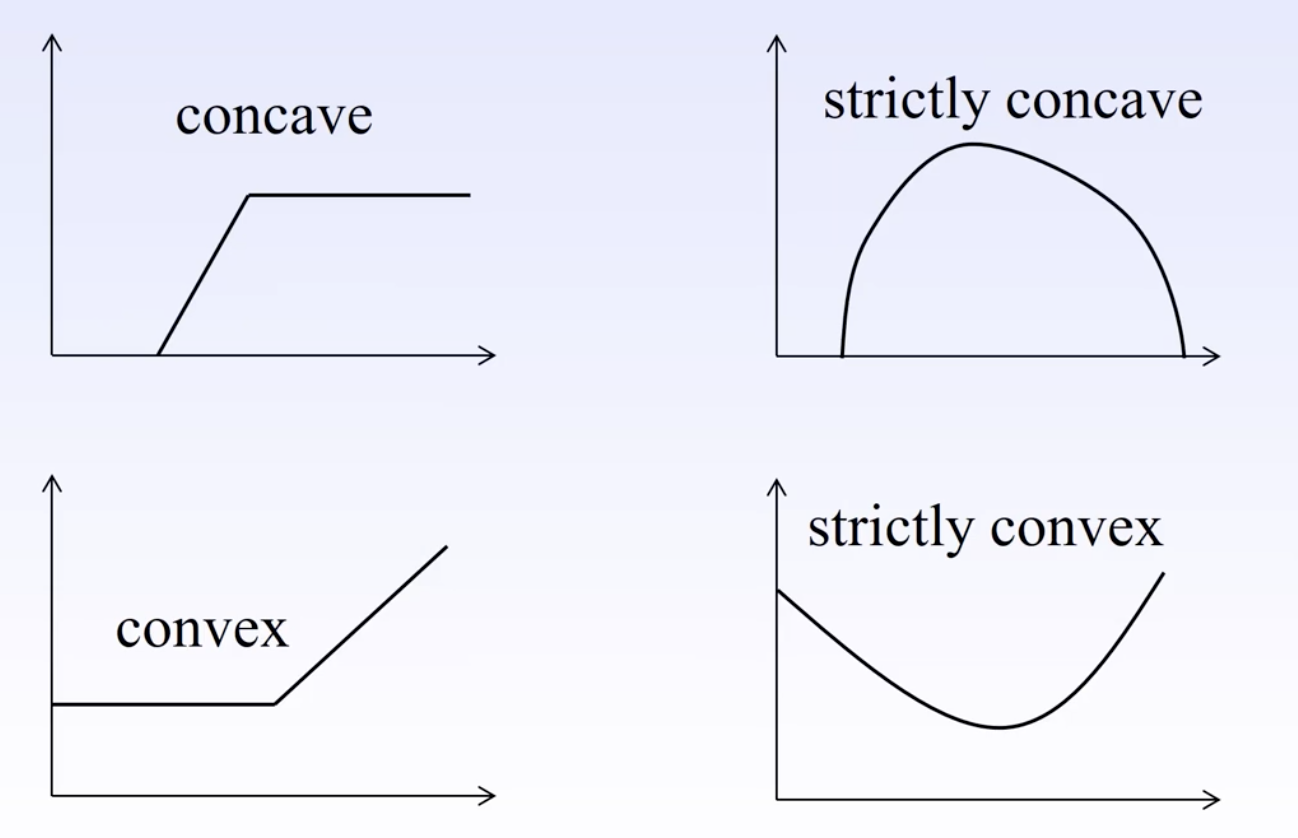
\includegraphics[width=0.9\textwidth]{imgs/concave_convex_graphs.png} \\
    \end{center}
\end{itemize}

\subsection{Smooth Functions}
\subsubsection{Smooth Functions in One Dimension}
\begin{itemize}
    \item Informal Definition: For a 1-D function from an interval to the real 
    line, if that function is twice continuously differentiable, then the
    function is:
    \begin{itemize}
        \item concave if and only if the second derivative is less than or equal
        to 0.
        \item concave if and only if the second derivative is less than 0. 
        \item convex if and only if the second derivative is greater than or 
        equal to 0.
        \item convex if and only if the second derivative is greater than 0.  
    \end{itemize}
    \item Formal Definition: If $ f : [a,b] \rightarrow \mathbb{R} $ is $ C^2 $, 
    then $ f $ is 
    \begin{itemize}
        \item concave $ \iff f'' \le 0 $ 
        \item strictly concave $ \iff f'' <  0 $ 
        \item convex $ \iff f'' \ge 0 $ 
        \item strictly convex $ \iff f'' >  0 $ 
    \end{itemize} 
\subsubsection{Conditions for Optimality in One Dimension Theorem}
\item Informal Definition: If we have a function that is once continuously 
differentiable, then for some value $ x^* $ in the inverval $ [a,b] $ such that 
$ f'(x^*) = 0 $ and $ f $ is:
\begin{itemize}
    \item concave, then $ x^* $ is a maxmium
    \item strictly concave, then $ x^* $ is the unique maxmium
    \item convex, then $ x^* $ is a minimum
    \item strictly convex, then $ x^* $ is the unique minimum
\end{itemize} 
\item Formal Definition: Consider a $ C^1 $ function $ f : [a,b] \rightarrow  
\mathbb{R} $, which satisfies $ f'(x^*) = 0 $ for some $ x^* \in [a,b] $. If $ f
$ is:
\begin{itemize}
    \item concave, then $ x^* $ is a maxmium
    \item strictly concave, then $ x^* $ is the unique maxmium
    \item convex, then $ x^* $ is a minimum
    \item strictly convex, then $ x^* $ is the unique minimum
\end{itemize} 

\subsubsection{Smooth Functions in Multiple Dimensions}
\begin{itemize}
    \item Formal Definition: If $ f : E \rightarrow \mathbb{R} $ is $ C^2 $
    \begin{itemize}
        \item $ f $ is concave $ \iff H_f $ is negative semidefinite
        \item $ f $ is strictly concave $ \iff H_f $ is negative definite
        \item $ f $ is convex $ \iff H_f $ is positive semidefinite
        \item $ f $ is strictly convex $ \iff H_f $ is positive definite 
    \end{itemize} 
\end{itemize}

\subsubsection{Conditions for Optimality in Multiple Dimension Theorem}
\item Informal Definition: If we have a function that is twice continuously 
differentiable, then for some convex set $ E \subset \mathbb{R}^N  $ where the 
first order condition is satisfied (the gradient at some point $ x^* $ is equal 
to the 0 vector) for some $ x^* \in E $, the function is
\begin{itemize}
    \item concave, then $ x^* $ is a maxmium
    \item strictly concave, then $ x^* $ is the unique maxmium
    \item convex, then $ x^* $ is a minimum
    \item strictly convex, then $ x^* $ is the unique minimum
\end{itemize} 
\item Formal Definition: Consider a $ C^2 $ function $ f : E \rightarrow  
\mathbb{R} $ for a convex set $ E \subset \mathbb{R}^N $, where $ f $ satisfies
$ \nabla f(x^*) = 0  $ for some $ x^* \in E $. If $ f
$ is:
\begin{itemize}
    \item concave, then $ x^* $ is a maxmium
    \item strictly concave, then $ x^* $ is the unique maxmium
    \item convex, then $ x^* $ is a minimum
    \item strictly convex, then $ x^* $ is the unique minimum
\end{itemize} 

\subsubsection{Lagrange Optimality Condition}
\item Informal Definition:
\item Formal Definition 

\end{itemize}

\end{document}
